% Chinese support

\documentclass[a4paper,twoside]{ctexart}
\usepackage{blindtext}  
\usepackage{geometry}


\ctexset{
	section={
		format+ = \zihao{-3} \heiti \raggedright,
		number = \chinese{section}
	}
}

% Page margin layout
\geometry{left=2.3cm,right=2cm,top=2.5cm,bottom=2.0cm}


\usepackage{listings}
\usepackage{xcolor}
\usepackage{geometry}
\usepackage{amsmath}
\usepackage{float}
\usepackage{hyperref}

\usepackage{graphics}
\usepackage{graphicx}
\usepackage{subfigure}
\usepackage{epsfig}
\usepackage{float}

\usepackage{circuitikz}
\usepackage{pbox}
\usepackage{bbding}
\newcommand{\ctikzlabel}[2]{\pbox{\textwidth}{#1\\#2}}


\usepackage{algorithm}
\usepackage[noend]{algpseudocode}

\usepackage{booktabs}
\usepackage{threeparttable}
\usepackage{longtable}
\usepackage{listings}
\usepackage{tikz}
\usepackage{multicol}

% cite package, to clean up citations in the main text. Do not remove.
\usepackage{cite}

\usepackage{color,xcolor}

%% The amssymb package provides various useful mathematical symbols
\usepackage{amssymb}
%% The amsthm package provides extended theorem environments
\usepackage{amsthm}
\usepackage{amsfonts}
\usepackage{enumerate}
\usepackage{enumitem}
\usepackage{listings}

\usepackage{pdfpages}

\usepackage{indentfirst}
\setlength{\parindent}{2em} % Make two letter space in the first paragraph
\usepackage{setspace}
\linespread{1.5} % Line spacing setting
\usepackage{siunitx}
\setlength{\parskip}{0.5em} % Paragraph spacing setting

% \usepackage[contents =22920202204622, scale = 10, color = black, angle = 50, opacity = .10]{background}

\renewcommand{\figurename}{图}
\renewcommand{\lstlistingname}{代码} 
\renewcommand{\tablename}{表格}
\renewcommand{\contentsname}{目录}
\floatname{algorithm}{算法}

\graphicspath{ {images/} }

%%%%%%%%%%%%%
\newcommand{\StudentNumber}{22920202204622}  % Fill your student number here
\newcommand{\StudentName}{熊恪峥}  % Replace your name here
\newcommand{\PaperTitle}{数字逻辑}  % Change your paper title here
\newcommand{\PaperType}{实验报告} % Replace the type of your report here
\newcommand{\Date}{2022年4月17日}
\newcommand{\College}{信息学院}
\newcommand{\CourseName}{数字逻辑}
%%%%%%%%%%%%%

%% Page header and footer setting
\usepackage{fancyhdr}
\usepackage{lastpage}
\pagestyle{fancy}
\fancyhf{}
% This requires the document to be twoside
\fancyhead[LO]{\texttt{\StudentName }}
\fancyhead[LE]{\texttt{\StudentNumber}}
\fancyhead[C]{\texttt{\PaperTitle }}
\fancyhead[R]{\texttt{第{\thepage}页,共\pageref*{LastPage}页}}


\title{\PaperTitle}
\author{\StudentName}
\date{\Date}

\lstset{
	basicstyle          =   \sffamily,          % 基本代码风格
	keywordstyle        =   \bfseries,          % 关键字风格
	commentstyle        =   \rmfamily\itshape,  % 注释的风格,斜体
	stringstyle         =   \ttfamily,  % 字符串风格
	flexiblecolumns,                % 别问为什么,加上这个
	numbers             =   left,   % 行号的位置在左边
	showspaces          =   false,  % 是否显示空格,显示了有点乱,所以不现实了
	numberstyle         =   \zihao{-5}\ttfamily,    % 行号的样式,小五号,tt等宽字体
	showstringspaces    =   false,
	captionpos          =   t,      % 这段代码的名字所呈现的位置,t指的是top上面
	frame               =   lrtb,   % 显示边框
}

\lstdefinestyle{PythonStyle}{
	language        =   Python, % 语言选Python
	basicstyle      =   \zihao{-5}\ttfamily,
	numberstyle     =   \zihao{-5}\ttfamily,
	keywordstyle    =   \color{blue},
	keywordstyle    =   [2] \color{teal},
	stringstyle     =   \color{magenta},
	commentstyle    =   \color{red}\ttfamily,
	breaklines      =   true,   % 自动换行,建议不要写太长的行
	columns         =   fixed,  % 如果不加这一句,字间距就不固定,很丑,必须加
	basewidth       =   0.5em,
}

\algnewcommand\algorithmicinput{\textbf{Input:}}
\algnewcommand\algorithmicoutput{\textbf{Output:}}
\algnewcommand\Input{\item[\algorithmicinput]}%
\algnewcommand\Output{\item[\algorithmicoutput]}%

\usetikzlibrary{positioning, shapes.geometric}

\newcommand{\ols}[1]{\mskip.5\thinmuskip\overline{\mskip-.5\thinmuskip {#1} \mskip-.5\thinmuskip}\mskip.5\thinmuskip}

% \usepackage{draftwatermark}
% \SetWatermarkText{22920202204622}
% \SetWatermarkScale{0.8}

\begin{document}
	
%%%%%%%%%%%%%%%%%%%%%%%%%%%%%%%%%%%%%%%%%%%%
\makeatletter % change default title style
\renewcommand*\maketitle{%
	\begin{center} 
		\bfseries  % title 
		{\LARGE \@title \par}  % LARGE typesetting
		\vskip 1em  %  margin 1em
		{\global\let\author\@empty}  % no author information
		{\global\let\date\@empty}  % no date
		\thispagestyle{empty}   %  empty page style
	\end{center}%
	\setcounter{footnote}{0}%
}
\makeatother
%%%%%%%%%%%%%%%%%%%%%%%%%%%%%%%%%%%%%%%%%%%%
	
	
\thispagestyle{empty}

\vspace*{1cm}

\begin{figure}[h]
	\centering
	
\includegraphics[width=4.0cm]{logo.png}
\end{figure}

\vspace*{1cm}

\begin{center}
	\Huge{\textbf{\PaperType}}
	
	\Large{\PaperTitle}
\end{center}

\vspace*{1cm}

\begin{table}[h]
	\centering	
	\begin{Large}
		\renewcommand{\arraystretch}{1.5}
		\begin{tabular}{p{3cm} p{5cm}<{\centering}}
			姓\qquad 名 & \StudentName  \\
			\hline
			学\qquad号 & \StudentNumber \\
			\hline
			日\qquad期 & \Date  \\
			\hline
			学\qquad院 & \College  \\
			\hline
			课程名称 & \CourseName  \\
			\hline
		\end{tabular}
	\end{Large}
\end{table}

\newpage

\title{
	\Large{\textcolor{black}{\PaperTitle}}
}
 
\newpage
\setcounter{page}{1}

\begin{spacing}{1.2}


\includepdf[pages={3,4}]{../instruction.pdf}
\setcounter{section}{3}

\section{实验结果}

对电路$F1$到$F8$进行测试,结果如表~\ref{{tbl:f12f8}}

\begin{table}[htbp]
	\centering
	\label{tbl:f12f8}
	\caption{电路$F1$到$F8$的测试结果}
	\begin{tabular}{c|cccccccccc}
		\toprule
		\hline
		A\hspace{1em} B&F1&F2&F3&F4&F5&F6&F7&F8&F9&F10\\
		\hline
		0\hspace{1em} 0&0&0&1&1&0&0&0&0&0&0\\
		0\hspace{1em} 0&0&1&1&0&1&1&0&0&1&0\\
		1\hspace{1em} 0&0&1&1&0&1&1&0&1&1&0\\
		1\hspace{1em} 1&1&1&0&0&0&1&1&0&1&1\\
		\hline
		\bottomrule
	\end{tabular}
\end{table}

其中\eqref{eqn:f5f7f9}是$F5$, $F7$, $F9$的与非式形式

\begin{equation}
	\label{eqn:f5f7f9}
	\begin{aligned}
		F5&=A\ols{B}+\ols{A}B \\
		&=\ols{\ols{A\ols{B}} \ols{\ols{A}B}} \\
		F7&=\ols{\ols{A}+\ols{B}} \\
		&=AB \\
		F9&=\ols{\ols{A}\ols{B}} \\
	\end{aligned}
\end{equation}

总线电路结果如表~\ref{tbl:bus}

\begin{table}[htbp]
	\centering
	\caption{电路$F1$到$F8$的测试结果}
	\label{tbl:bus}
	\begin{tabular}{cccc|c}
		\toprule
		\hline
		1A&1E&2A&2E&B\\
		\hline
		0&0&0&1&0\\
		0&0&1&1&0\\
		1&0&0&1&1\\
		1&0&1&1&1\\
		0&1&0&0&0\\
		0&1&1&0&1\\
		1&1&0&0&0\\
		1&1&1&0&1\\
		\hline
		$\times$&1&$\times$&1&高阻(0)\\
		\hline
		\bottomrule
	\end{tabular}
\end{table}

\section{思考题}

\begin{enumerate}
	\item 与非门、或非门中的多余输入端该如何处理,如不进行处理,让它们悬空将会产
	生什么结果?

	TTL与非门多余输入端悬空相当于输入1,对输出没有影响,但考虑到抗干扰,应该接高电平或者与其他变量并联使用。
	
	TTL或非门多余输入端悬空相当于输入1,对输出结果有影响,因此应当接地或者与其他变量并联使用。

	\item 图 1.2(b)中 1E、2E 能不能同时为“0”,为什么?
	
	当1E, 2E同时为0, 会直接连接两门的输出端,这是不允许的。
\end{enumerate}

\clearpage


\includepdf[pages={6}]{../instruction.pdf}
\setcounter{section}{4}

\section{电路设计}

\subsection{表决器电路}

\subsubsection{逻辑表达式}

依题意,三个与三个以上为$1$时输出$F=1$。逻辑表达式如\eqref{eqn:voting}


注意到$\overline{AC}$出现了两次,所以$F$可以用8个与非门完成。

\subsubsection{电路设计}

根据以上分析,设计电路如图~\ref{fig:voting}

\begin{figure}[h]
	\centering
	\begin{minipage}{0.48\linewidth}
		\caption{投票电路}
		\label{fig:voting}
		\centering
		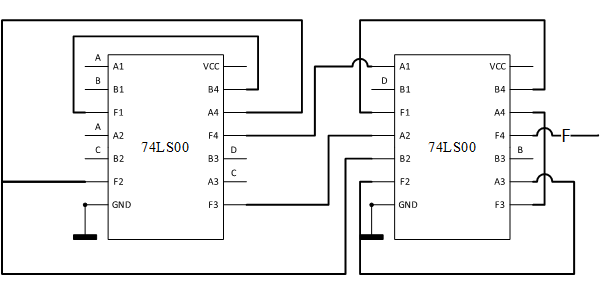
\includegraphics[width=\textwidth]{fig1.png}
	\end{minipage}
	~
	\begin{minipage}{0.48\linewidth}
		\centering
		\begin{equation}
			\label{eqn:voting}
			\begin{aligned}
				F&=ABC+ABD+ACD+BCD \\
				&=(AB+AC)D+(AC+CD)B \\
				&=\ols{\ols{\ols{\ols{AB}\cdot\ols{AC}}\cdot D}\cdot \ols{\ols{\ols{AC}\cdot\ols{CD}}\cdot B } }
			\end{aligned}
		\end{equation}
	\end{minipage}
\end{figure}

\subsubsection{实验结果}

按照图~\ref{fig:voting}连接电路,得到图~\ref{fig:res21}

\begin{figure}[h]
	\centering
	\caption{实际电路连接}
	\label{fig:res21}
	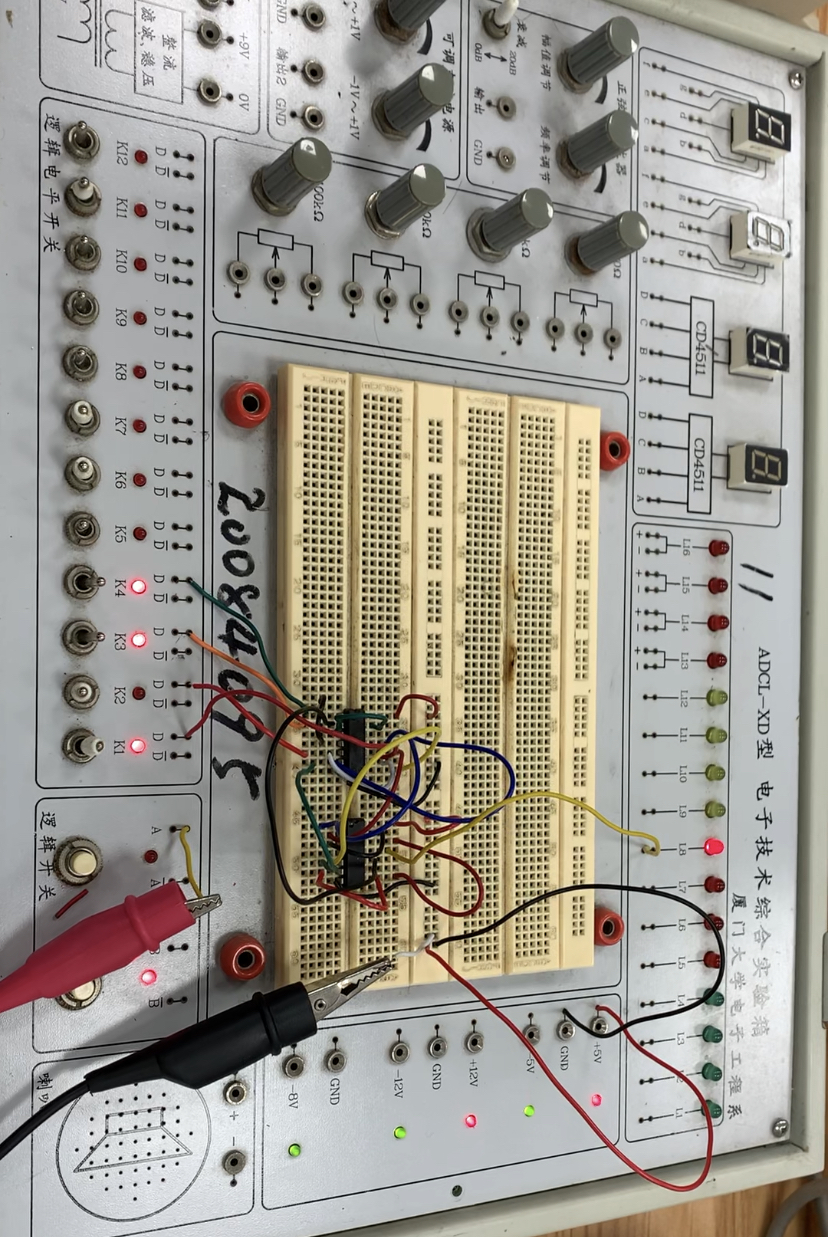
\includegraphics[width=0.48\textwidth,angle=90,origin=c]{fig_res21.png}
\end{figure}


\subsection{比较器电路}

\subsubsection{逻辑表达式}

根据题意可以得到真值表表~\ref{tbl:cmp}。并根据表~\ref{tbl:cmp}可以列出表达式\eqref{eqn:cmp}。

\begin{table}[H]
	\centering
	\begin{minipage}{0.48\linewidth}
		\centering
		\caption{真值表}
		\label{tbl:cmp}
		\begin{tabular}{cccc|ccc}
			\toprule
			\hline
			$A_2$&$A_1$&$B_2$&$B_1$&$P_1$&$P_2$&$P_3$ \\
			\hline
			0&0&0&0&0&1&0 \\
			0&0&0&1&0&0&1 \\
			0&0&1&0&0&0&1 \\
			0&0&1&1&0&0&1 \\
			0&1&0&0&1&0&0 \\
			0&1&0&1&0&1&0 \\
			0&1&1&0&0&0&1 \\
			0&1&1&1&0&0&1 \\
			1&0&0&0&1&0&0 \\
			1&0&0&1&1&0&0 \\
			1&0&1&0&0&1&0 \\
			1&0&1&1&0&0&1 \\
			1&1&0&0&1&0&0 \\
			1&1&0&1&1&0&0 \\
			1&1&1&0&1&0&0 \\
			1&1&1&1&0&1&0 \\
			\hline
			\bottomrule
		\end{tabular}
	\end{minipage}
	~
	\begin{minipage}{0.48\linewidth}
		\begin{equation}
			\label{eqn:cmp}
			\begin{aligned}
				P_1&=A_1B_1+(A_1B_1+\ols{A_1} \ols{B_1})A_0B_0 \\
				&=\ols{\ols{A_1\ols{B_1}}\cdot \ols{A_0\ols{B_0}\cdot\ols{\ols{A_1}B_1} } }\\
				P_2&=(A_1B_1+\ols{A_1}\ols{B_1})(A_0B_0+\ols{A_0}\ols{B_0}) \\
				&= \ols{\ols{\ols{P_1\cdot1}\ols{P_3\cdot1}}\cdot 1}\\
				P_3&=(\ols{A_1}B_1)+(A_1B_1+\ols{A_1}\ols{B_1})\ols{A_0}B_0\\
				&=\ols{\ols{\ols{A_1}B_1}\cdot \ols{\ols{A_0}B_0\cdot\ols{A_1\ols{B_1}} } }\\
			\end{aligned}
		\end{equation}
	\end{minipage}
\end{table}

\subsubsection{电路图}

根据表达式画出逻辑电路图如图~\ref{fig:cmp}

\begin{figure}[H]
	\centering
	\caption{比较器电路}
	\label{fig:cmp}
	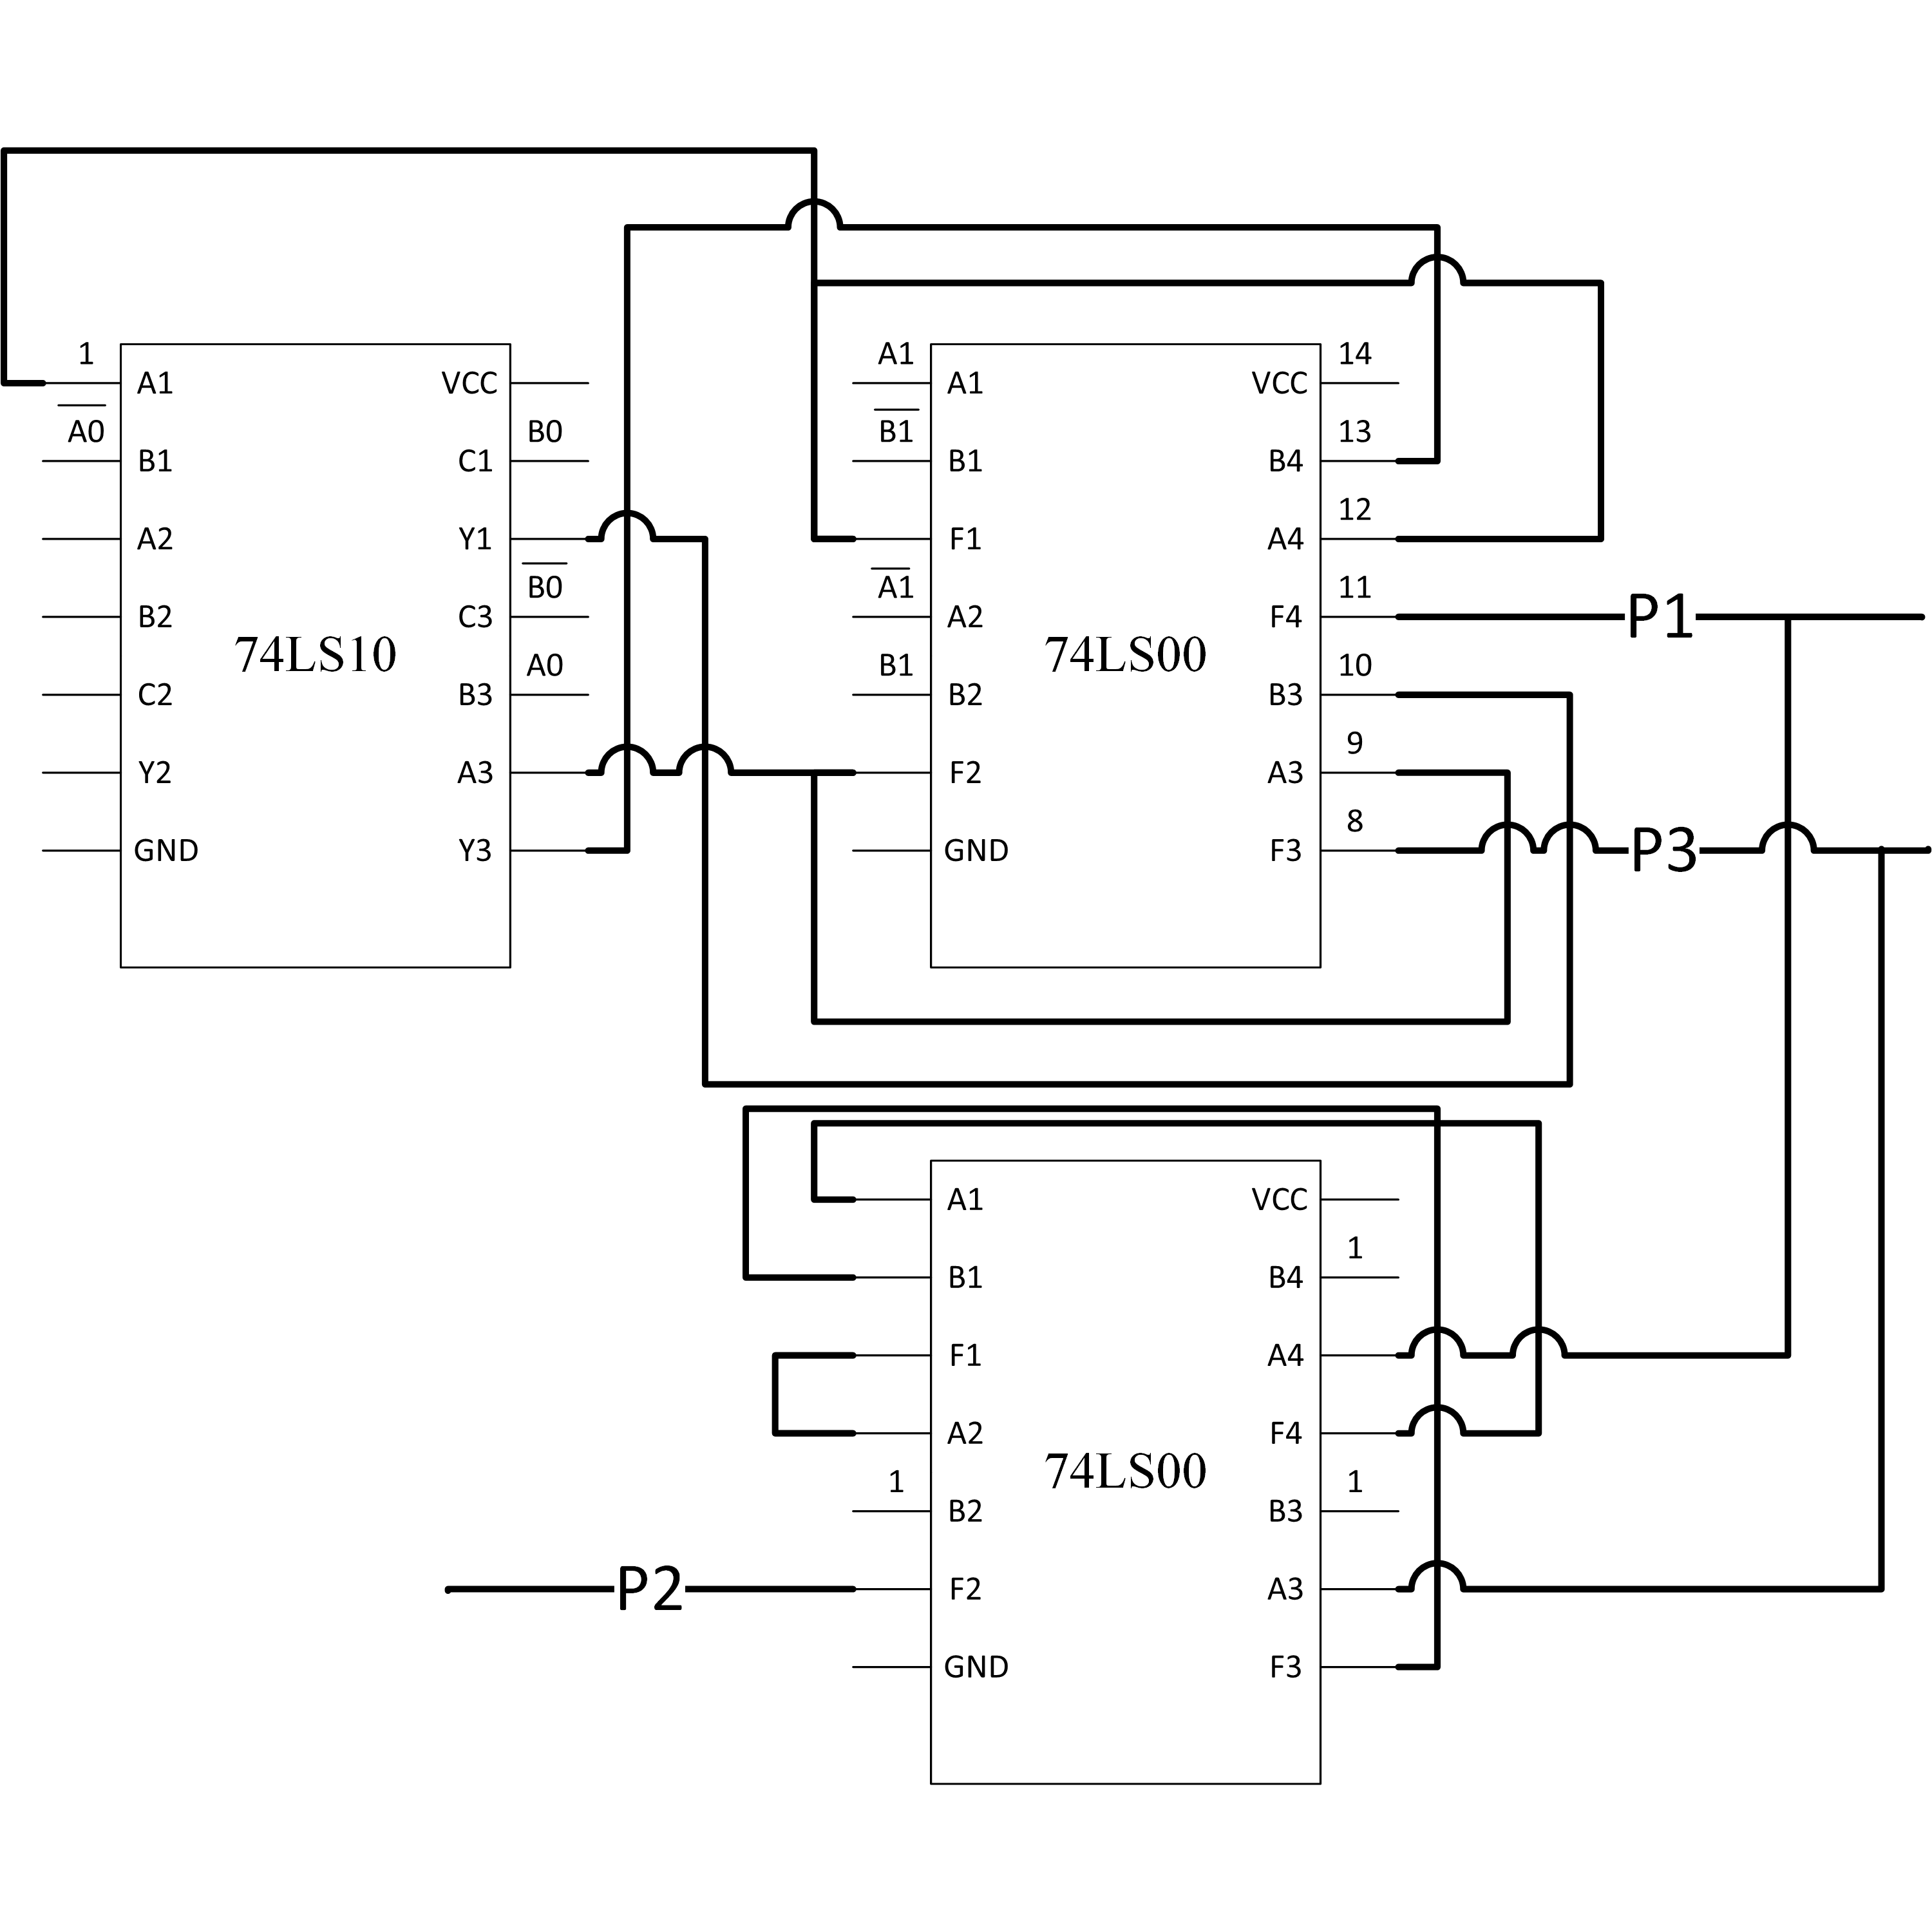
\includegraphics[width=0.5\textwidth]{fig2.png}
\end{figure}

\subsubsection{实验结果}

按照图~\ref{fig:cmp}连接电路得到图~\ref{fig:res22},并将输出接入LED灯,
观察到现象如表~\ref{tbl:cmpres}所示。

\begin{figure}[htbp]
	\centering
	\begin{minipage}{0.48\linewidth}
		\caption{实验结果}
		\label{tbl:cmpres}
		\begin{tabular}{cccc|ccc|c}
			\toprule
			\hline
			$A_2$&$A_1$&$B_2$&$B_1$&$P_1$&$P_2$&$P_3$&实验现象 \\
			\hline
			0&0&0&0&0&1&0&中间灯亮 \\
			0&0&0&1&0&0&1&右灯亮 \\
			0&0&1&0&0&0&1&右灯亮 \\
			0&0&1&1&0&0&1&右灯亮 \\
			0&1&0&0&1&0&0&左灯亮 \\
			0&1&0&1&0&1&0&中间灯亮 \\
			0&1&1&0&0&0&1&右灯亮 \\
			0&1&1&1&0&0&1&右灯亮 \\
			1&0&0&0&1&0&0&左灯亮 \\
			1&0&0&1&1&0&0&左灯亮 \\
			1&0&1&0&0&1&0&中间灯亮 \\
			1&0&1&1&0&0&1&右灯亮 \\
			1&1&0&0&1&0&0&左灯亮 \\
			1&1&0&1&1&0&0&左灯亮 \\
			1&1&1&0&1&0&0&左灯亮 \\
			1&1&1&1&0&1&0&中间灯亮 \\
			\hline
			\bottomrule
		\end{tabular}
	\end{minipage}
	~
	\begin{minipage}{0.48\linewidth}
		\centering
		\caption{实际电路连接}
		\label{fig:res22}
		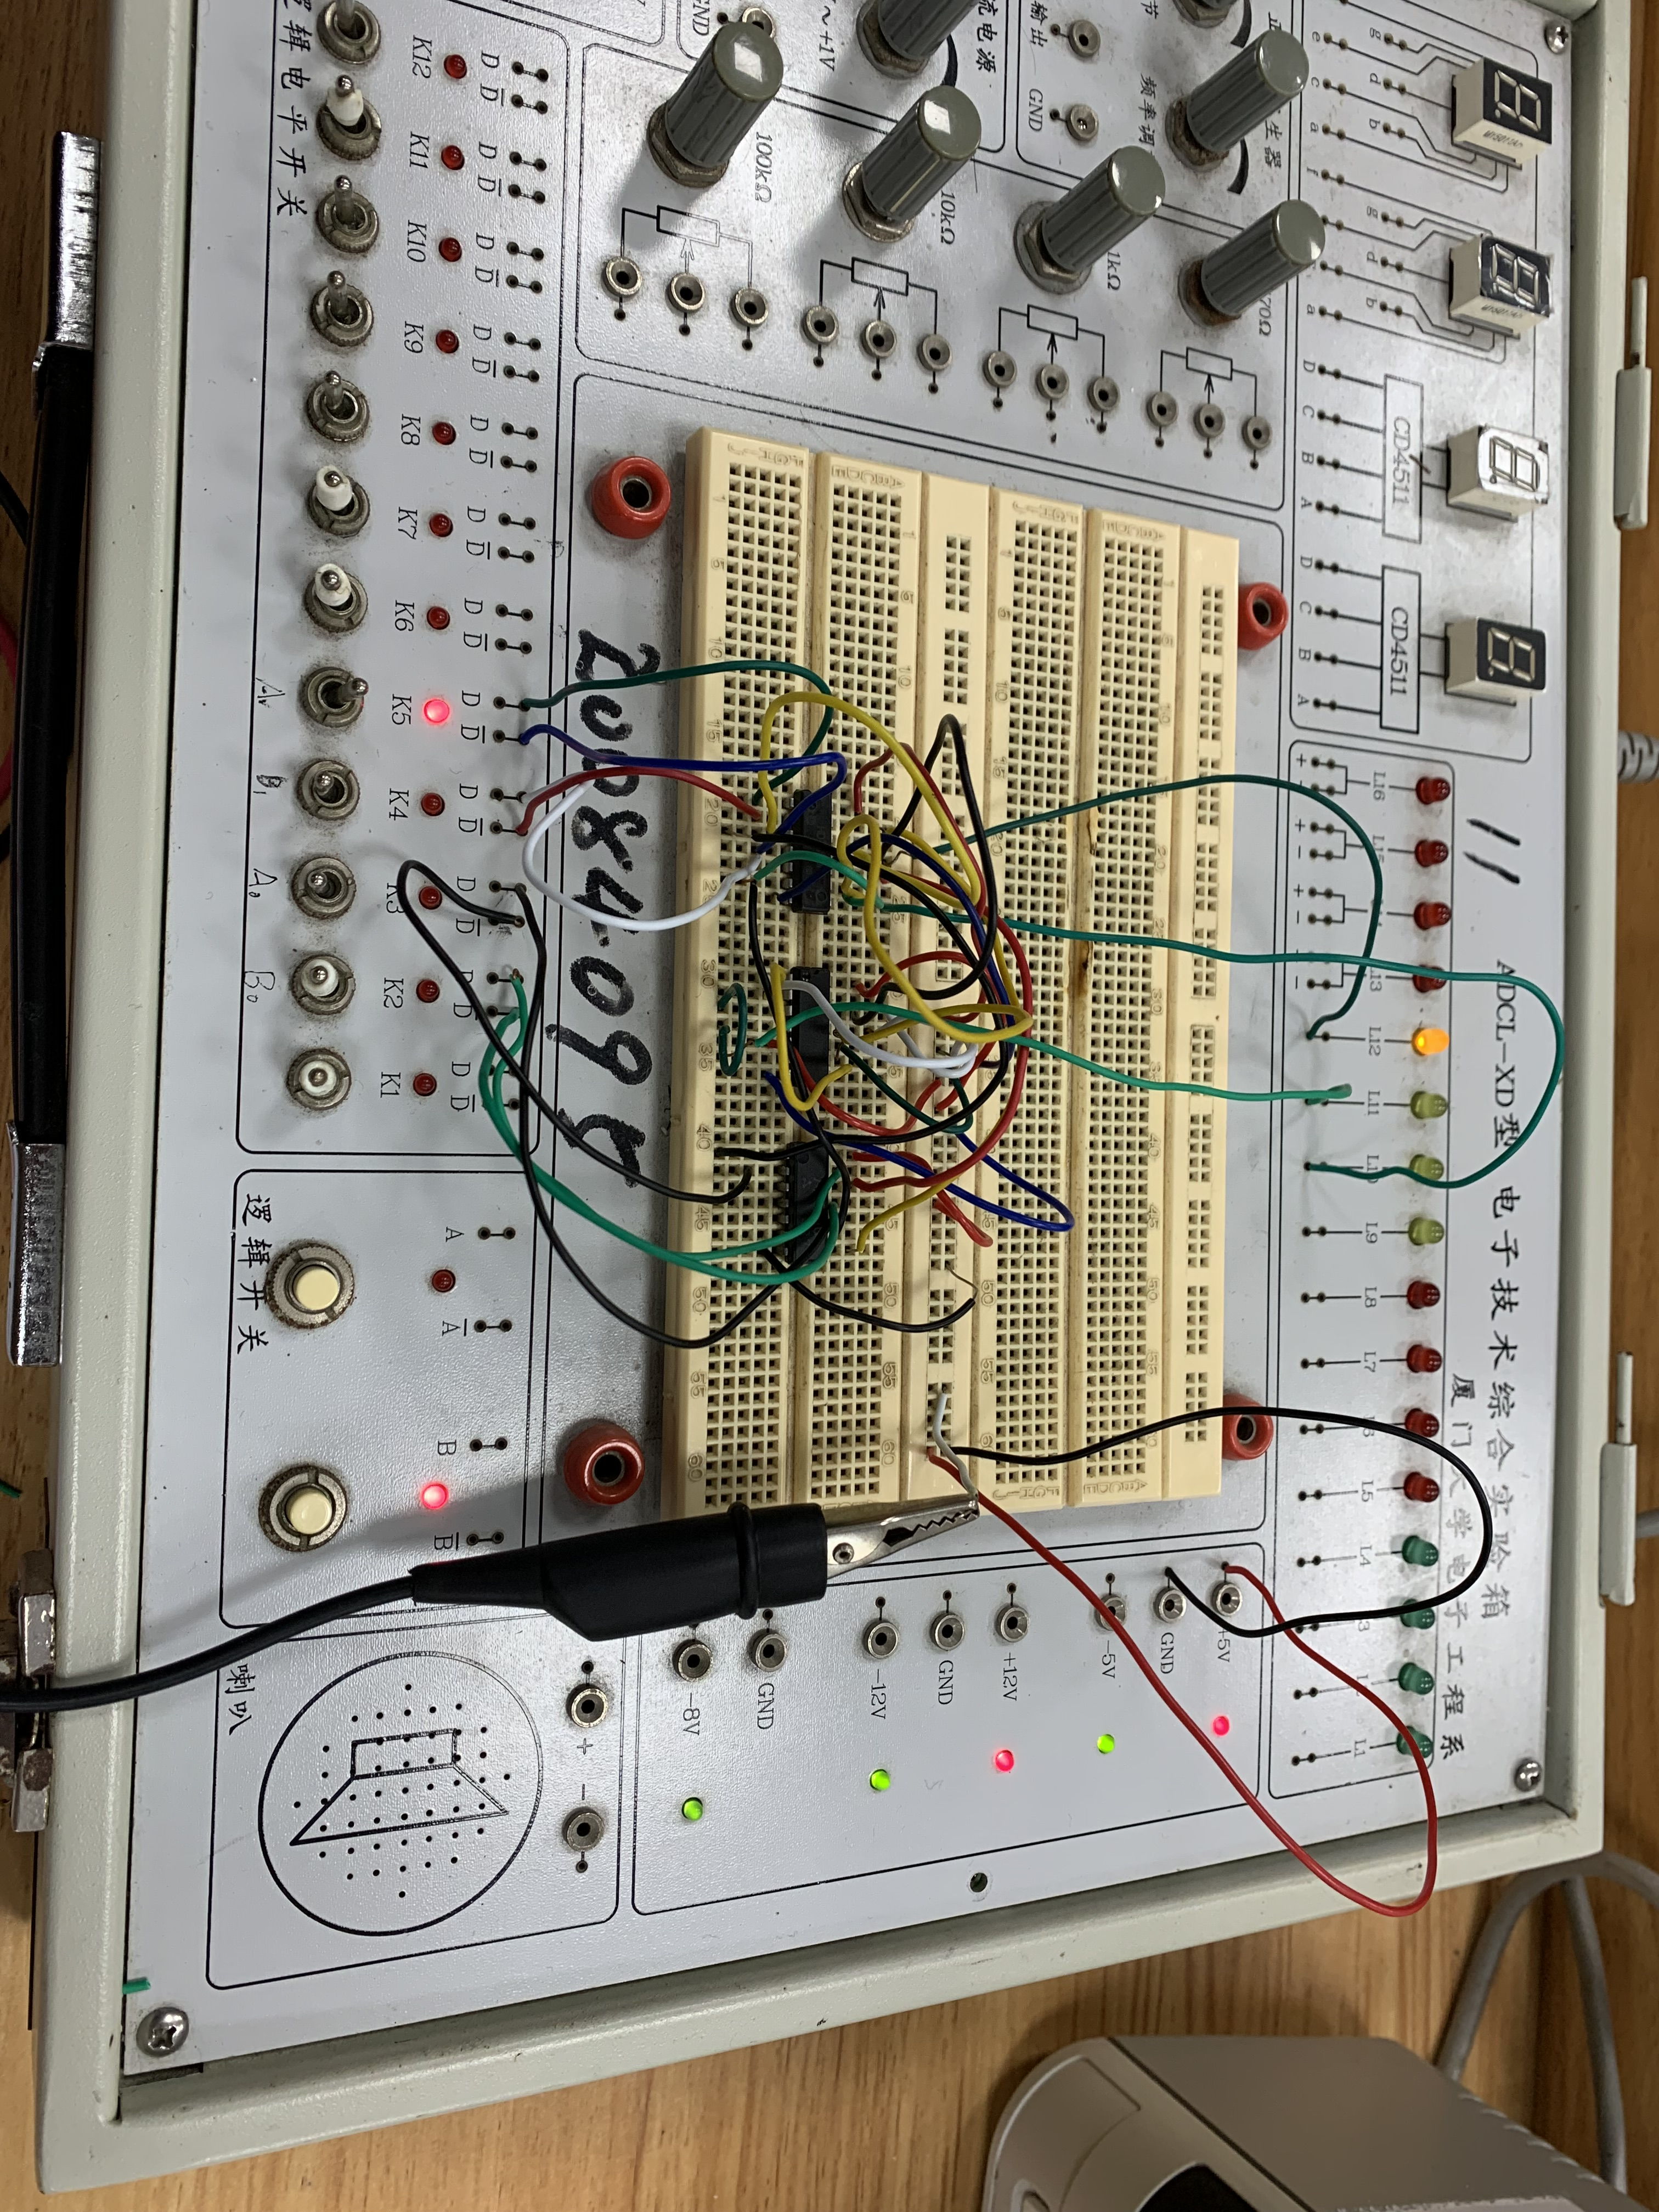
\includegraphics[width=0.9\textwidth,angle=90,origin=c]{fig_res22.jpg}
	\end{minipage}
\end{figure}

\section{思考题}

\begin{enumerate}
	\item 上述两个电路用摩根定理进行逻辑变换为用与非门实现的形式后,使用芯片的个数、类
	型是否减少?为什么?

	使用芯片的类型确实会减少。类型减少是很显然的。直接写出的表达式一般由与运算和或运算组成,
	但化为与非式之后只有与非一种操作,可以减少门的种类。
	
	使用芯片数量可能减少。如\eqref{eqn:voting}中化为与非式找到了一项被多个与非项
	包含了,这把理论上的9个门降低到了8个。又如\eqref{eqn:cmp}中,化为与非式之后
	出现了3变量与非项,可以借助3输入与非门实现进而减少一个门。然而确实可以举出
	反例,如\eqref{eqn:invexample}。这个简单的逻辑函数化为与非式之后没有减少
	门的数量。
	\begin{equation}
		\label{eqn:invexample}
		\begin{aligned}
			F&=A+B\\
			&=\ols{\ols{A}\ols{B}}
		\end{aligned}
	\end{equation}
\end{enumerate}

\end{spacing}

\end{document}